% \ifdefined\ishandout
%\documentclass[xcolor={usenames, table, x11names}, handout, 10pt]{beamer} 
% \usepackage{pgfpages}
% \pgfpagesuselayout{2 on 1}[a4paper,border shrink=5mm]
% \else
% \ifdefined\isNote
% \documentclass[xcolor={usenames, table, x11names}, final, 10pt]{beamer} 
% \setbeameroption{show only notes}
% \else
% \ifdefined\isDraft
% \documentclass[xcolor={usenames, table, x11names}, draft, 10pt]{beamer} 
% \else
% \documentclass[xcolor={usenames, table, x11names}, final, 10pt]{beamer} 
% \fi
% \fi
% \fi

\documentclass[10pt]{beamer}

% final/draft cambia velocità compilazione. Anche "handout" è ammesso
%\usepackage{etex}% serve per caricare dopo tikz, richiesto da chemfig
% http://tex.stackexchange.com/questions/7896/no-room-for-a-new-dimen-when-including-tikz
%\setbeamercolor{emph}{fg=red}
%\renewcommand<>{\emph}[1]{%
%  {\usebeamercolor[fg]{emph}\only#2{\itshape}#1}%
%}
\usetheme[]{Feather}
\usepackage[polutonikogreek,italian]{babel} % parole in greco antico polutonikogreek (lez 01)
\usepackage[utf8x]{inputenc}
\usepackage[T1]{fontenc}


 

% \mode<presentation>
% {%
%   % [compress] lascia una riga coi pallini sola in cima
%   \usecolortheme{seahorse}% crane=giallo, beetle: il bianco/nero in alto non si legge 
%   % wolverine_mistogialloblu
%   % \usefonttheme[onlylarge]{structuresmallcapsserif}
%   % \usefonttheme[onlysmall]{structurebold}
%   \setbeamercolor{emph}{fg=red}
%   \setbeamerfont{title}{shape=\itshape, family=\rmfamily}
%   % \setbeamercolor{title}{fg=red!80!black}
%   % \setbeamercolor{title}{fg=red!80!black,bg=red!20!white}
%   \setbeamertemplate{footline}[frame number]{}
%   % \setbeamertemplate{navigation symbols}[vertical]
%   % la riga sotto toglie le iconcine di navigazione in basso che non funzionano
%   \setbeamertemplate{navigation symbols}{} 
%   \setbeamercovered{transparent}
%   \useinnertheme{rounded}% mette le palline al posto dei quadrati
%   \setbeamertemplate{blocks}[rounded][shadow=true] %aggiunge l'ombra ai blocchi
%   % \setbeamercolor{background canvas}{bg=black!20}
%   \setbeamercolor{section in head/foot}{fg=black, bg=blue!10}
%   \setbeamertemplate{section in head/foot shaded}[default][40]
%   %% le due righe sopra cambiano il colore della striscia in alto, la headline
%   \setbeamertemplate{headline}{%
%     \leavevmode%
%     \hbox{%
%       \begin{beamercolorbox}[wd=\paperwidth,ht=5ex,dp=1ex]{section in head/foot}%
%         \insertsectionnavigationhorizontal{\paperwidth}{}{\hskip0pt plus1filll}
%         \insertsubsectionnavigationhorizontal{\paperwidth}{\hskip0pt plus1filll}{}
%       \end{beamercolorbox}%
%     }
%   }
% }%% fine del mode presentation
% \mode<handout>
% {%
%   % Questo pezzo makeatother serve per mettere le pagine e il nome sul
%   % pie' di pagina
%   \makeatother
%   \setbeamertemplate{footline}
%   {
%     \leavevmode%
%     \hbox{%
%       \begin{beamercolorbox}[wd=.2\paperwidth,ht=2.25ex,dp=1ex,center]{author in head/foot}%
%         \usebeamerfont{author in head/foot}\insertshortauthor
%       \end{beamercolorbox}%
%       \begin{beamercolorbox}[wd=.8\paperwidth,ht=2.25ex,dp=1ex,center]{title in head/foot}%
%         \usebeamerfont{title in head/foot}
%         Chimica del suolo. Scienze vivaistiche, ambiente e gestione del
%         verde\hspace*{3em}
%         \input{AnnoAccademico.txt} pag.
%         \insertframenumber{} %attiva questo per i numeri di pagina ma fa casino 
%       \end{beamercolorbox}}%
%     \vskip0pt%
%   }
%   \makeatletter
%   \setbeamercolor{background canvas}{bg=red!5}
% }





% http://zyliu2005.blogspot.com/2008/08/latex-change-mrow-color-of-table.html
% se non si mette "xcolor" in questo modo, pdflatex fa casino
%\usepackage[x11names]{xcolor} % richiesto per colortbl
\usepackage{color} % richiesto per ambiente picture linee a colori
\usepackage{graphics} % legge i file pdf jpg jpeg png
\usepackage{siunitx}% serve per \celsius e le unita di misura

% fine delle unità di misura speciali
% \usepackage[final]{pdfpages} % per mettere pdf a pagine multiple (lez 01)
%\usepackage[version=4]{mhchem} % 26 feb 2015: mail con martin hensel
% necessario mchem.sty da lui inviato per \ce{Na, Ca, Ba,} le virgole

% \usepackage{xymtexpdf}
% \usepackage{chmst-pdf}

% \usepackage{xymtex}
% \usepackage[chemist]{chemtimes}
\usepackage{xmpmulti} %serve per overlay dei grafici
\usepackage{graphicx}
% \usepackage{booktabs} % \toprule \midrule \bottomrule nelle tabelle (lez 01)
\usepackage{multirow} % righe in tabelle 
\usepackage{tabularx}
\usepackage{array} % richiesto per colorare e definire colonne e per
% dcolumn
\usepackage{dcolumn} % serve per allineare le colonne sulle virgole
\usepackage{ulem} % sottolineature e overstrike
%\usepackage{chemfig, xstring} % chiama tikz xstring lez 11
% \usepackage{gensymb} % serve per \celsius dopo passaggio a wheezy (lez 01)
% \usepackage{rotating}% per ruotare figure
\usepackage{hyperref} %serve al pacchetto multimedia sotto
\usepackage{multimedia} % per animazioni in file esterni
% \usepackage{media9} % per animazioni in file esterni
% http://latex-community.org/forum/viewtopic.php?f=45&t=20581
% \usepackage{amsmath} % serve per le equazioni anche chimiche 

\usepackage{multicol}% per spezzare gli indici in due colonne. riga
% 135
%% \pgfdeclareimage[height=1cm]{logo}{DIPSA_BN.eps}
%% \logo{\pgfuseimage{logo}}
% \logo{\includegraphics[width=0.5cm]{DIPSA_BN.jpg}}

\usepackage{textcomp} % serve per il segno permille \textperthousand lez 09
% \usepackage{../mol2chemfig} %%lez 11
% \usepackage{animate} % serve per le animazioni lez 11
% \usepackage{tabu} %per colorare il testo delle tabelle, non lo sfondo lez 11

% \mathversion{boldchem}
%\newchemenvironment{chemalign}{align}
%\newchemenvironment{chemalign*}{align*}
% \newchemenvironment{chemalignat}{alignat}
\newcolumntype{,}{D{,}{,}{2}}
%% http://tex.stackexchange.com/questions/13423/how-to-change-the-color-of-href-links-for-real
\definecolor{links}{HTML}{FF00FF}
% FF00FF magenta, FF0000 rosso. bluastro 2A1B81
% http://www.color-hex.com/color-names.html
\hypersetup{colorlinks,linkcolor=,urlcolor=links}
%% 2 righe sopra da lez 01
% \newcommand{\greco}[1]{% per scrivere direttamente in greco
% \begin{otherlanguage*}{greek}#1\end{otherlanguage*}}
%\newcommand*\circleatom[1]{\tikz\node[circle,draw,fill=green!30]{\printatom{#1}};
%}

\newcommand{\chref}[2]{
  \href{#1}{{\usebeamercolor[bg]{Feather}#2}}
}

\DeclareMathSizes{12}{30}{16}{12}
\title{25 anni di conduzione Biologica in area Mediterranea}% \input{NomeDelCorso.txt}}
\author{\input{autore.txt}}
\institute{\input{DISPAA.txt}}
% \date{\input{AnnoAccademico.txt}}

% \usetikzlibrary{positioning, calc, snakes} %serve per la legge di Bragg
% \showboxdepth= 5
% \showboxbreadth= 5
% \overfullrule = 2cm
\subtitle{\textbf{Uno
studio di fisica del suolo}}

\begin{document}
\begin{frame}<beamer:1|handout:0>[plain, noframenumbering]
  \titlepage 
\end{frame}

% presumo che queste righe mettano dei segnali in ogni parte e sezione
\AtBeginPart{\frame<beamer>{\partpage
    \transsplitverticalout[duration=1] 
    \begin{block}{}
      % \tableofcontents[subsectionstyle=show]
      \tableofcontents[subsectionstyle=hide]
    \end{block}
  }}

\AtBeginSection[]{\frame<beamer>{%
    \begin{block}{}
      \tableofcontents[currentsection, subsectionstyle=hide]
    \end{block}
  }
}

\begin{frame}
  \frametitle{Obiettivi}
  \large
  \begin{itemize}[<+->]
  \item verificare la presenza di differenze nelle caratteristiche
    fisiche del suolo in aree: \newline coltivate convenzionalmente
    (\emph{CO}) \newline oppure \newline coltivate  a biologico (\emph{OO}) tramite;
    \begin{itemize}
    \item Densit\`a apparente
      \begin{itemize}
      \item Metodo \emph{Core}
      \item Metodo \emph{Clod}
      \end{itemize}
    \item Stabilit\`a degli aggregati
    \item Distribuzione della porosit\`a      
    \end{itemize}
  \item verificare eventuali effetti dovuti a diverse lavorazioni
    (aratura, rippatura, frangizollatura).
  \end{itemize}
\end{frame}



\part{Densit\`a apparente}
\section{Metodo \emph{Core}}
\begin{frame}
  \frametitle{Metodo \emph{Cored}} %\citep{ugolini2010basi} 
  \begin{columns}
    \column{.50\textwidth}
    \begin{block}{}
      \pause
      \begin{itemize}[<+->] 
      \item Estrazione di un volume di suolo noto
        ($V_{iniz}=854.1 cm^3$) mediante un cilindro non deformabile
        di ottone
      \item vagliatura a \SI{2}{\milli\meter}
      \item misura volume scheletro per spinta idrostatica
        ($V_{scheletro}$)
      \item essiccamento in stufa a 105$^o$C e pesatura della terra
        fine ($P_{secco}$)
      \item calcolo densit\`a apparente sottraendo al volume del
        cilindro il volume dello scheletro
      \end{itemize}
    \end{block}
    \column{.48\textwidth}
       \only<2>{
         \begin{figure}[ht]
           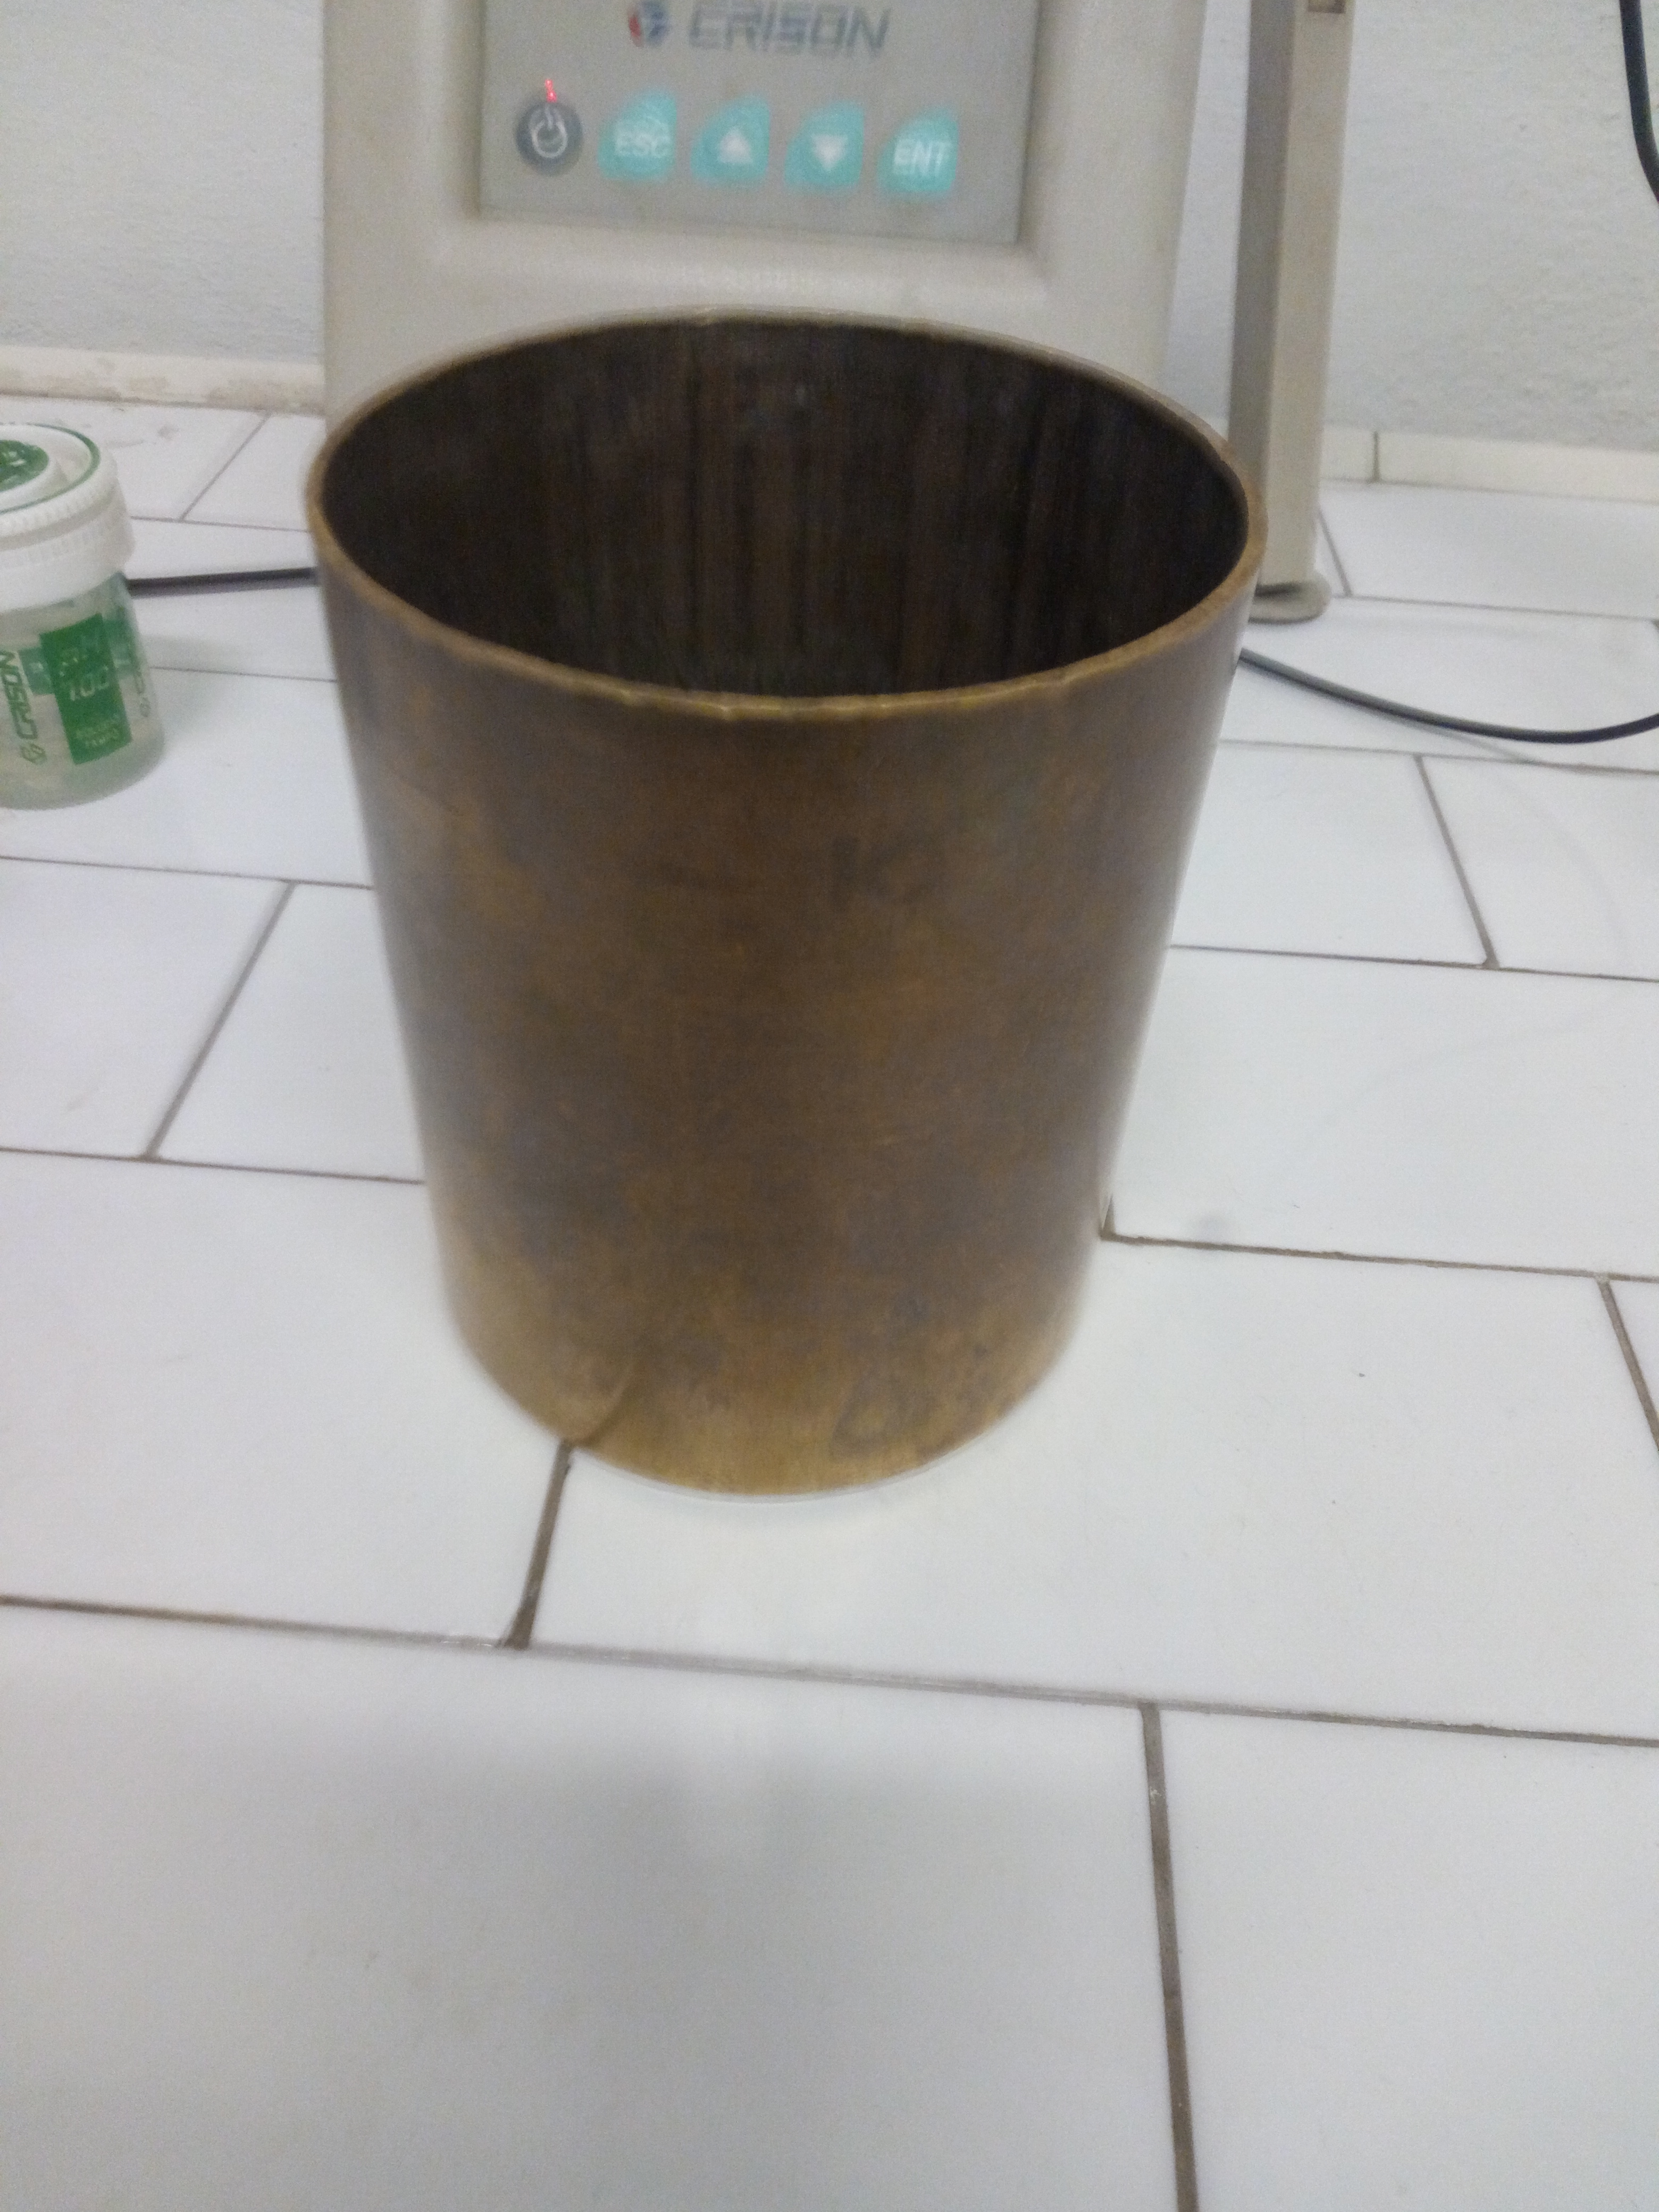
\includegraphics[width=0.8\textwidth]{../foto/cilindroOttone.jpeg}
      \end{figure}}
    \only<3>{
      \begin{figure}[ht]
        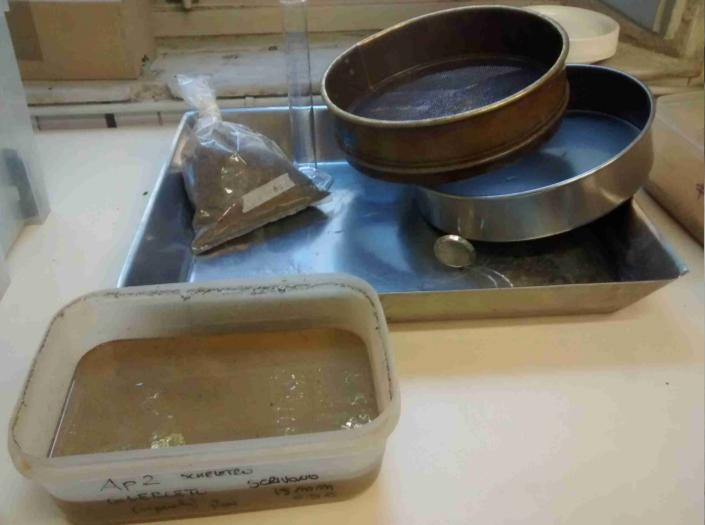
\includegraphics[width=0.8\textwidth]{../foto/strum.jpeg}
      \end{figure}
    }
    \only<5>{
      \begin{figure}[ht]
        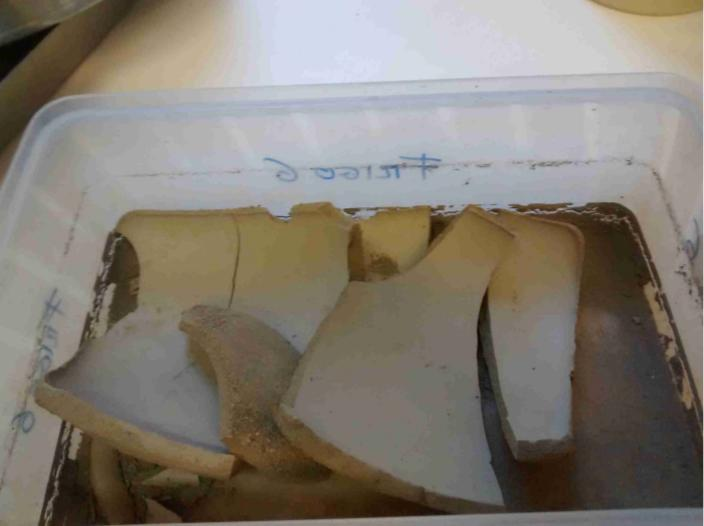
\includegraphics[width=0.8\textwidth]{../foto/secco.jpeg}
      \end{figure}
    }

    \only<6>{
      \begin{center}
        \[
        D_{App}=\frac{P_{secco}}{V_{iniz}-V_{scheletro}}
        \]
      \end{center}
    }
  \end{columns}  
\end{frame}

\begin{frame}
  \frametitle{Sintesi tramite modello lineare}
  \transwipe<4>[direction=90]
  \begin{columns}
    \column{.60\textwidth}
    \pause
    \begin{itemize}
      \onslide<2->\item 
      \vspace{0.25cm}
      $Y \sim \mu + \beta_1x_1 + \beta_2x_2 + \beta_3x_3 + \epsilon$
      \vspace{0.25cm}

      in cui le variabili categoriche sono:
      \begin{itemize}
        \onslide<2->\item $\beta_1$  anno \newline 2015, 2016
        \onslide<2->\item $\beta_2$ conduzione \newline convenzionale (CO), biologico (OO)
        \onslide<2->\item $\beta_3$ lavorazioni \newline arato, rippato, frangizollato
      \end{itemize}
      \onslide<3->\item validazione del modello attraverso l'analisi dei residui    
      \onslide<4->\item analisi della varianza (ANOVA)
      \only<4-> {\begin{table}
          \centering
          \footnotesize
          \begin{tabular}{lrrrrr}
            \hline
            & Df & Sum Sq & Mean Sq & F value & Pr($>$F) \\ 
            \hline
            Anno & 1 & 0.05 & 0.05 & 4.36 & 0.0395 \\ 
            Conduzione & 1 & 0.05 & 0.05 & 4.68 & 0.0332 \\ 
            Lavorazione & 2 & 0.01 & 0.00 & 0.26 & 0.7702 \\ 
            Residui & 90 & 0.97 & 0.01 &  &  \\ 
            \hline
          \end{tabular}
          \label{tab:Anova densita campo 2015-2016}
        \end{table}}

    \end{itemize}
    \column{.38\textwidth}
    \only<3>{\includegraphics[width=\textwidth]{../grafici/density/plot_2anni.pdf}}
    
  \end{columns}
\end{frame}


% \begin{frame}
%   \begin{figure}
%     \includegraphics[width=0.8\textwidth]{../grafici/density/secondabozza-GrafDensitaCampo_1}
%   \end{figure}
% \end{frame}

\begin{frame}
  \footnotesize
  % latex table generated in R 3.4.0 by xtable 1.8-2 package
  % Thu Jun 22 15:19:10 2017
  \begin{table}[ht]
    \centering
    \begin{tabular}{lllccc}
      \hline
      Anno & Conduzione & Lavorazione & Densit\`a apparente
                                        ($g/cm^3$) & dev std & n \\ 
      \hline
      2015 & CO & Ara & 1.35 & 0.14 &   5 \\ 
           &    & Fzo & 1.34 & 0.07 &   5 \\ 
           &    & Rip & 1.38 & 0.10 &   5 \\ 
           & OO & Ara & 1.37 & 0.10 &  15 \\ 
           &    & Fzo & 1.44 & 0.10 &  15 \\ 
           &    & Rip & 1.43 & 0.07 &  15 \\ 
      \\
      2016 & CO & Ara & 1.38 & 0.16 &   6 \\ 
           &    & Fzo & 1.35 & 0.15 &   6 \\ 
           &    & Rip & 1.26 & 0.09 &   5 \\ 
           & OO & Ara & 1.37 & 0.06 &   6 \\ 
           &    & Fzo & 1.35 & 0.07 &   6 \\ 
           &    & Rip & 1.40 & 0.15 &   6 \\ 
      \hline
    \end{tabular}
    \label{tab:RiassuntoDensitaCAmpo}
  \end{table}
\end{frame}

\begin{frame}
  \begin{figure}[ht]
    \includegraphics[width=0.8\textwidth]{../grafici/density/boxplot_2anni.pdf}
  \end{figure}
\end{frame}

\begin{frame}
  % latex table generated in R 3.4.0 by xtable 1.8-2 package
  % Thu Jun 22 16:16:27 2017
  \begin{table}[ht]
    \centering
    \begin{tabular}{lrrrrr}
      \hline
      & Df & Sum Sq & Mean Sq & F value & Pr($>$F) \\ 
      \hline
      Anno & 1 & 0.05 & 0.05 & 4.36 & 0.0395 \\ 
      Conduzione & 1 & 0.05 & 0.05 & 4.68 & 0.0332 \\
      \textbf<2>{Lavorazione} & \textbf<2>{2} & \textbf<2>{0.01} & \textbf<2>{0.00} &\textbf<2>{0.26} & \textbf<2>{0.7702} \\ 
      Residui & 90 & 0.97 & 0.01 &  &  \\ 
      \hline
    \end{tabular}
    \label{tab:Anova densita campo 2015-2016}
  \end{table}
\end{frame}

% \begin{frame}
%   \begin{figure}[ht]
%     \includegraphics[width=0.8\textwidth]{../grafici/density/plot_2anni.pdf}
%   \end{figure}
% \end{frame}

\begin{frame}{t table densit\`a grandi volumi}
  % latex table generated in R 3.4.0 by xtable 1.8-2 package
  % Fri Jun 23 11:16:03 2017
  \begin{table}[ht]
    \centering
    \begin{tabular}{rrrrr}
      \hline
      &Estimate & Std. Error & t value & Pr($>$$|$t$|$) \\ 
      \hline
      Convenzionale 2015 & 1.36  & 0.02 & 62.28 & 0.00 \\ 
      Convenzionale 2016 & -0.03 & 0.02 & -1.52 & 0.13 \\ 
      Biologico 2015     &  0.05  & 0.02 &  2.18 & 0.03 \\ 
      \hline
    \end{tabular}
    \label{tab:Riassunto densit`a campo 2015 e 2016}
  \end{table}
  \begin{block}{\emph{Scostamenti!}}
    La prima riga riporta il valore del trattamento \emph{corner}
    (1.36 $g/cm^3$).

    Le altre righe riportano invece il valore dello scostamento (e
    relativo t-test) rispetto al trattamento \emph{corner}.

    Di conseguenza il trattamento biologico 2016 ha come valore assoluto
    1.36 - 0.03 + 0.05 =  1.38 $g/cm^3$.
  \end{block}
\end{frame}


\begin{frame}
  \begin{figure}[ht]
    \includegraphics[width=0.8\textwidth]{../grafici/density/boxplot_2annitrt.pdf}
  \end{figure}
\end{frame}





\section{Piccoli aggregati di 3-5 cm di diametro}

\begin{frame}{Procedura}
  \begin{columns}
    \column{.50\textwidth}
    \begin{block}{Su un singolo aggregato \newline 3-5 cm di diametro:}  
      \pause
      \begin{itemize}[<+->]
      \item lasciato per una notte a bagno nel petrolio
        \footnotesize{(densit\`a $D_{petrolio}=0.761g/cm^3$)}
      \item asciugato \textit{“a brillantezza”}
      \item misura del peso $P_{petrolio}$ del volume di petrolio
        spostato dall'aggregato, ovvero della spinta idrostatica
      \item  calcolo del volume dell'aggregato
      \item essiccazione a $150^oC$ per una notte e pesatura campione
        secco ($P_{150}$)
      \item calcolo della densit\`a apparente
      \end{itemize}
    \end{block}
    \column{.48\textwidth}

    \only<2-3>{
      \begin{figure}[ht]
        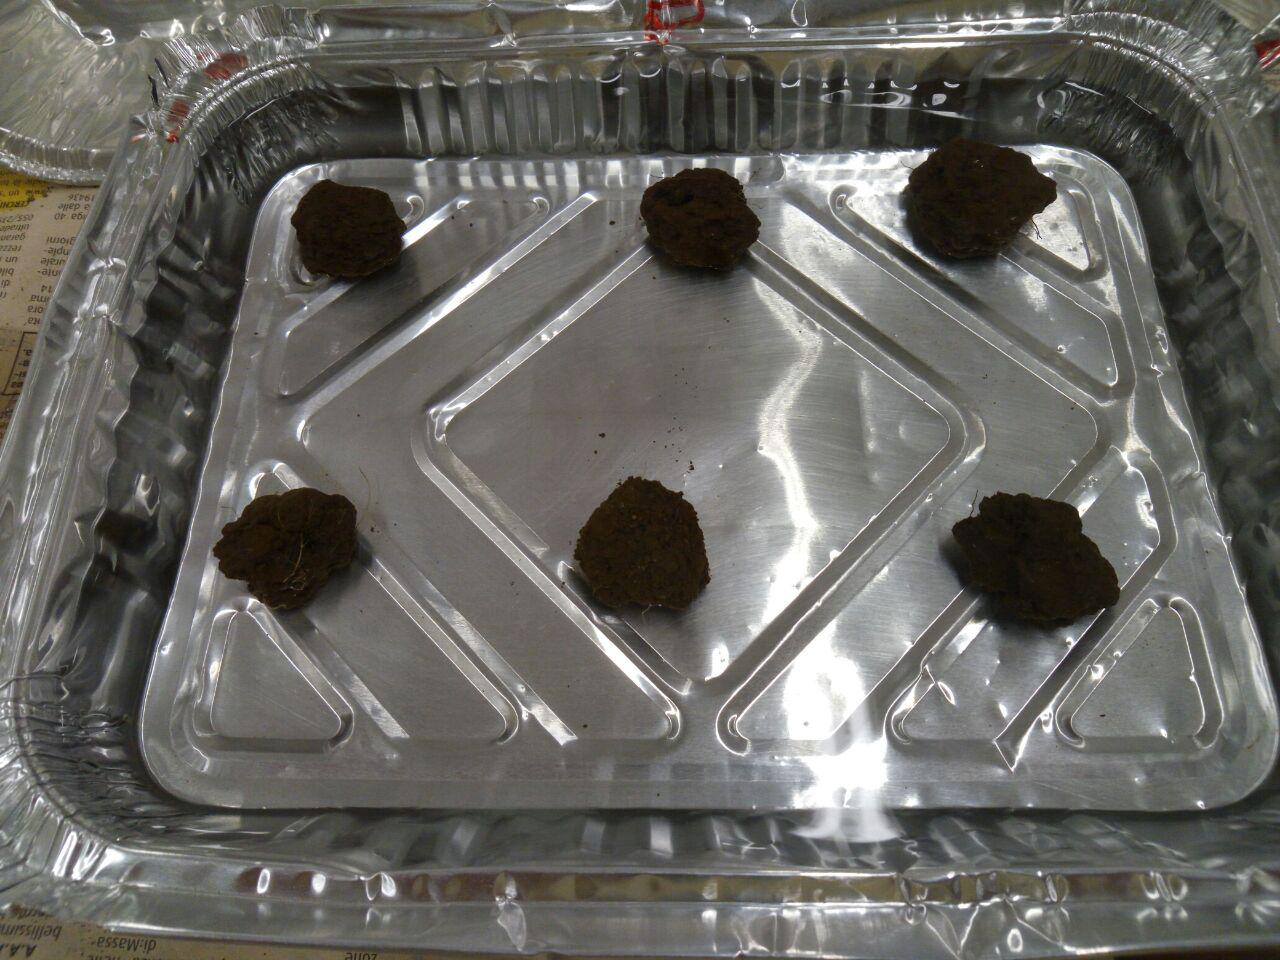
\includegraphics[width=0.8\textwidth]{../foto/petrolio.jpeg}
      \end{figure}
    }
    \only<4>{
      \begin{figure}[ht]
        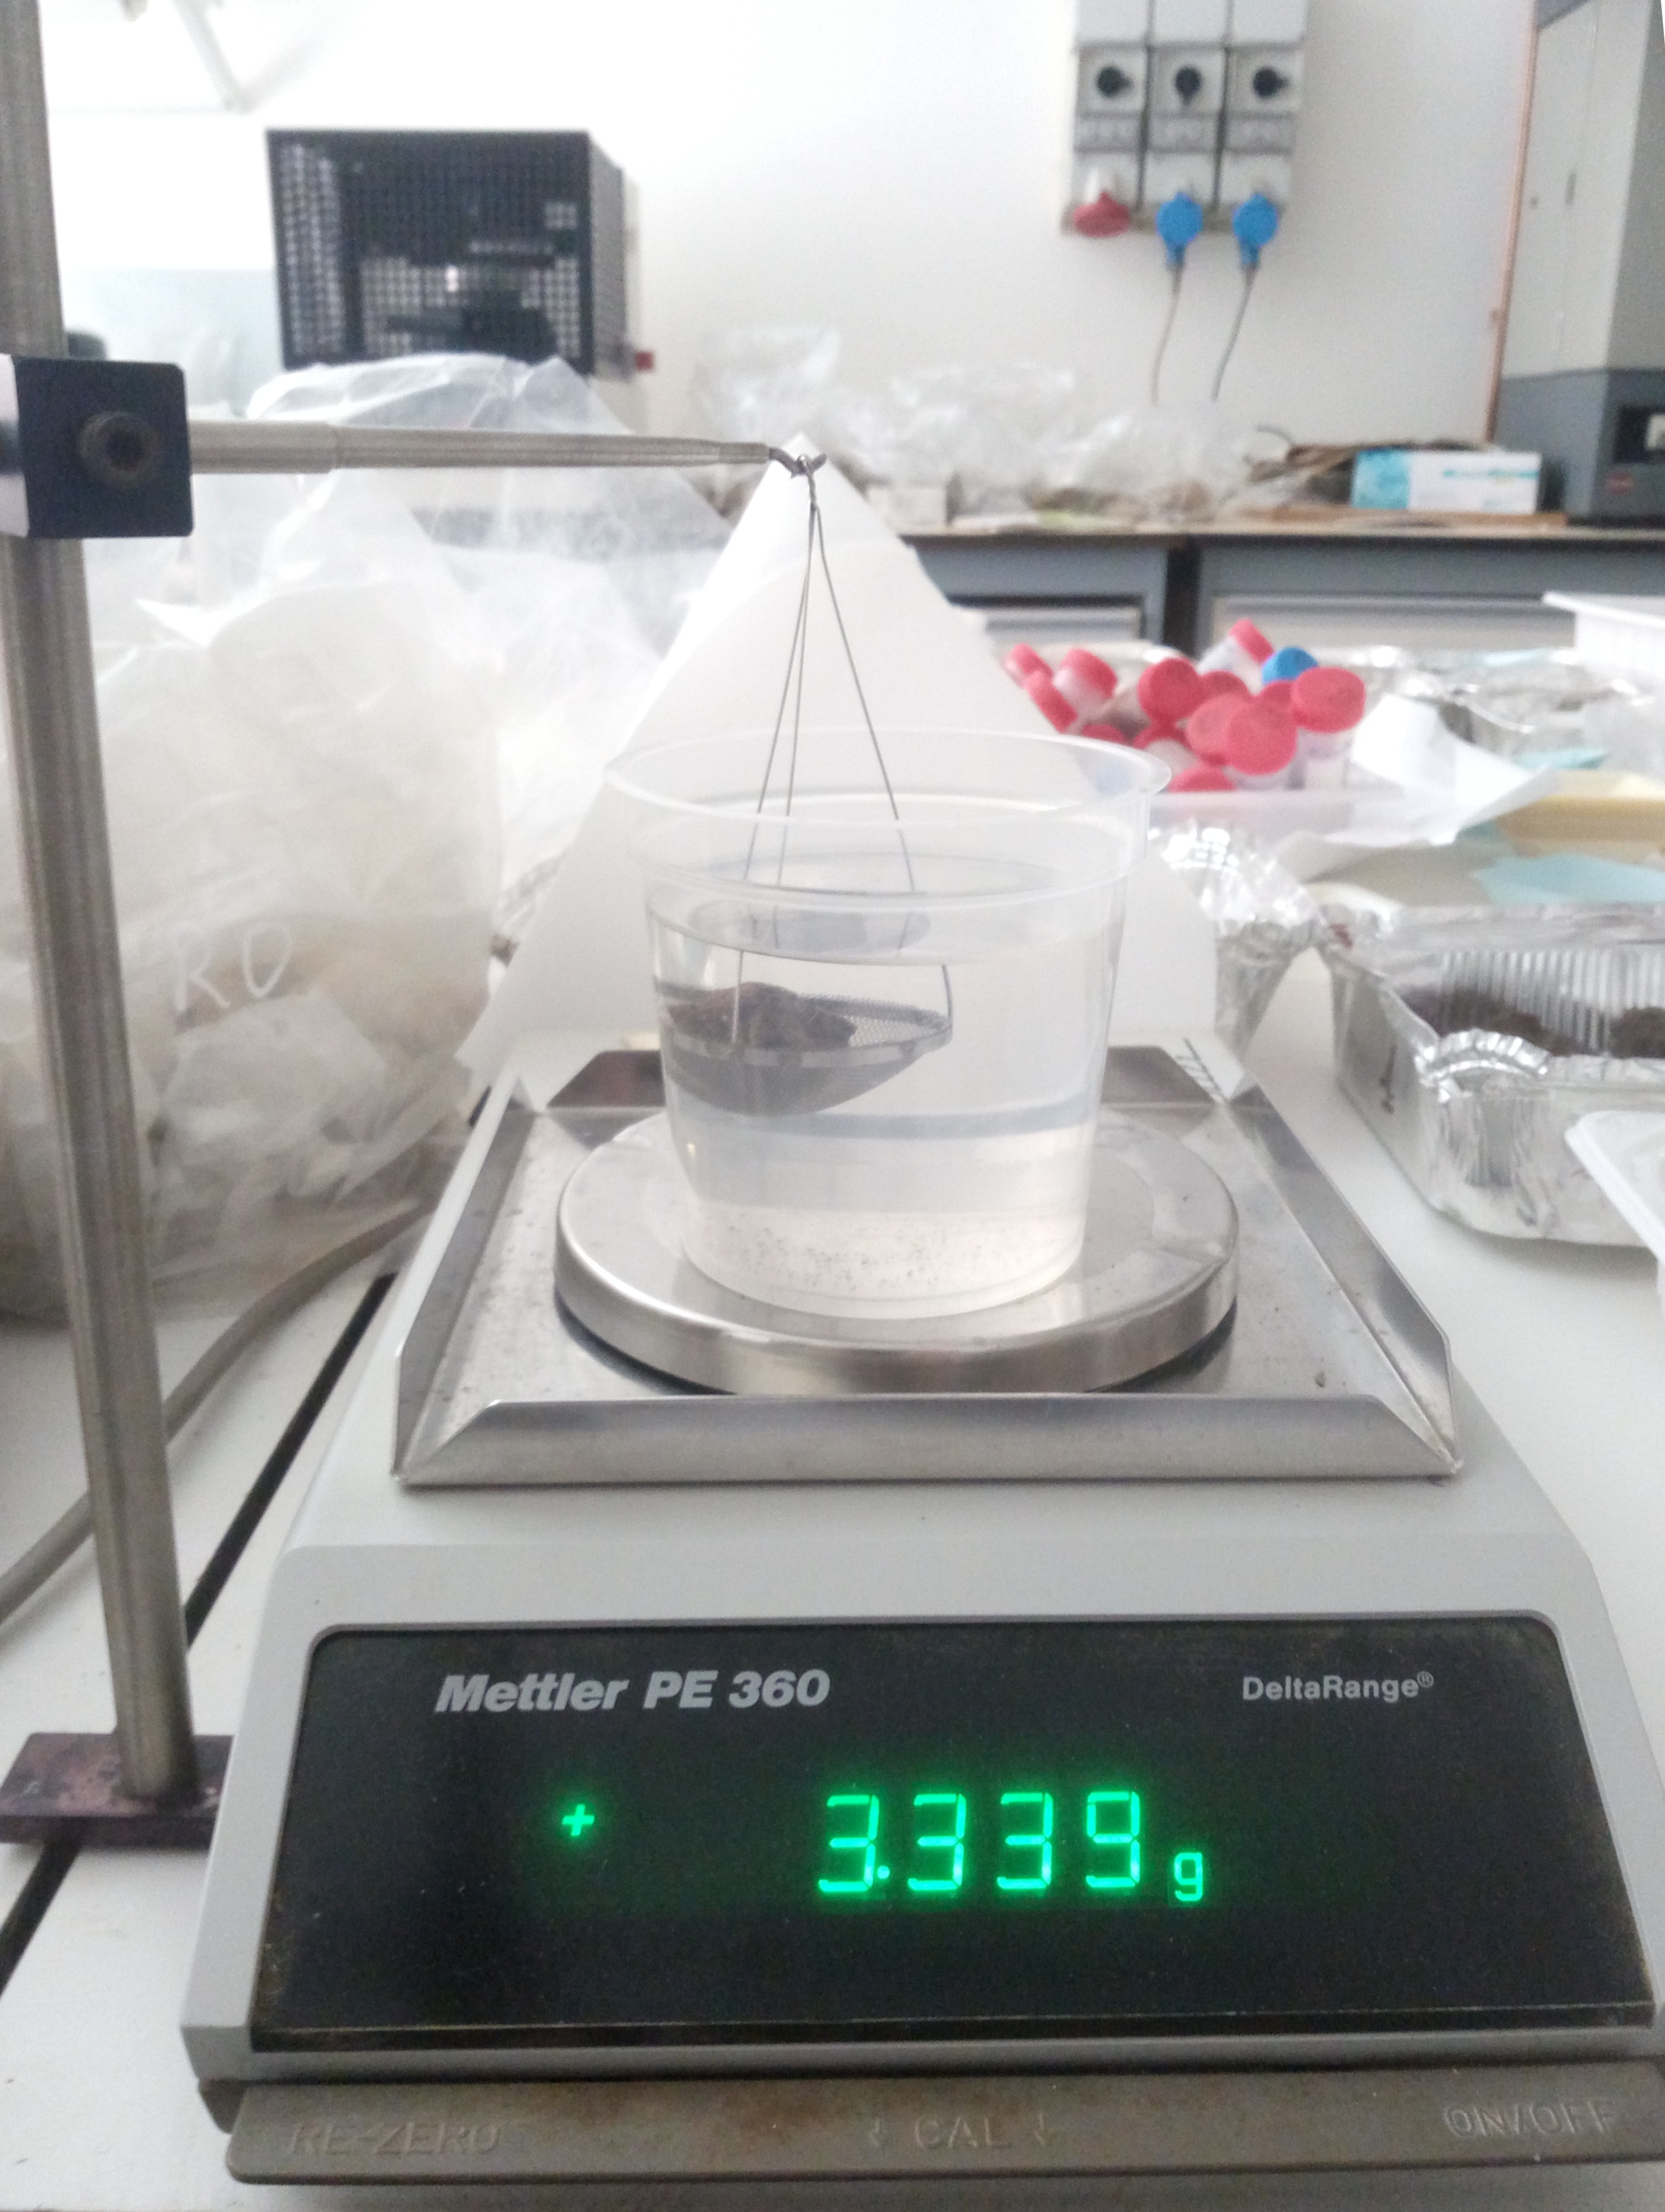
\includegraphics[width=0.8\textwidth]{../foto/navicella.jpeg}
      \end{figure}
    }
    \only<5>{
      \begin{center}
        \[
        V_{aggregato}=\frac{P_{petrolio}}{D_{petrolio}}
        \]
      \end{center}
      
    }
    \only<6>{
      \begin{figure}[ht]
        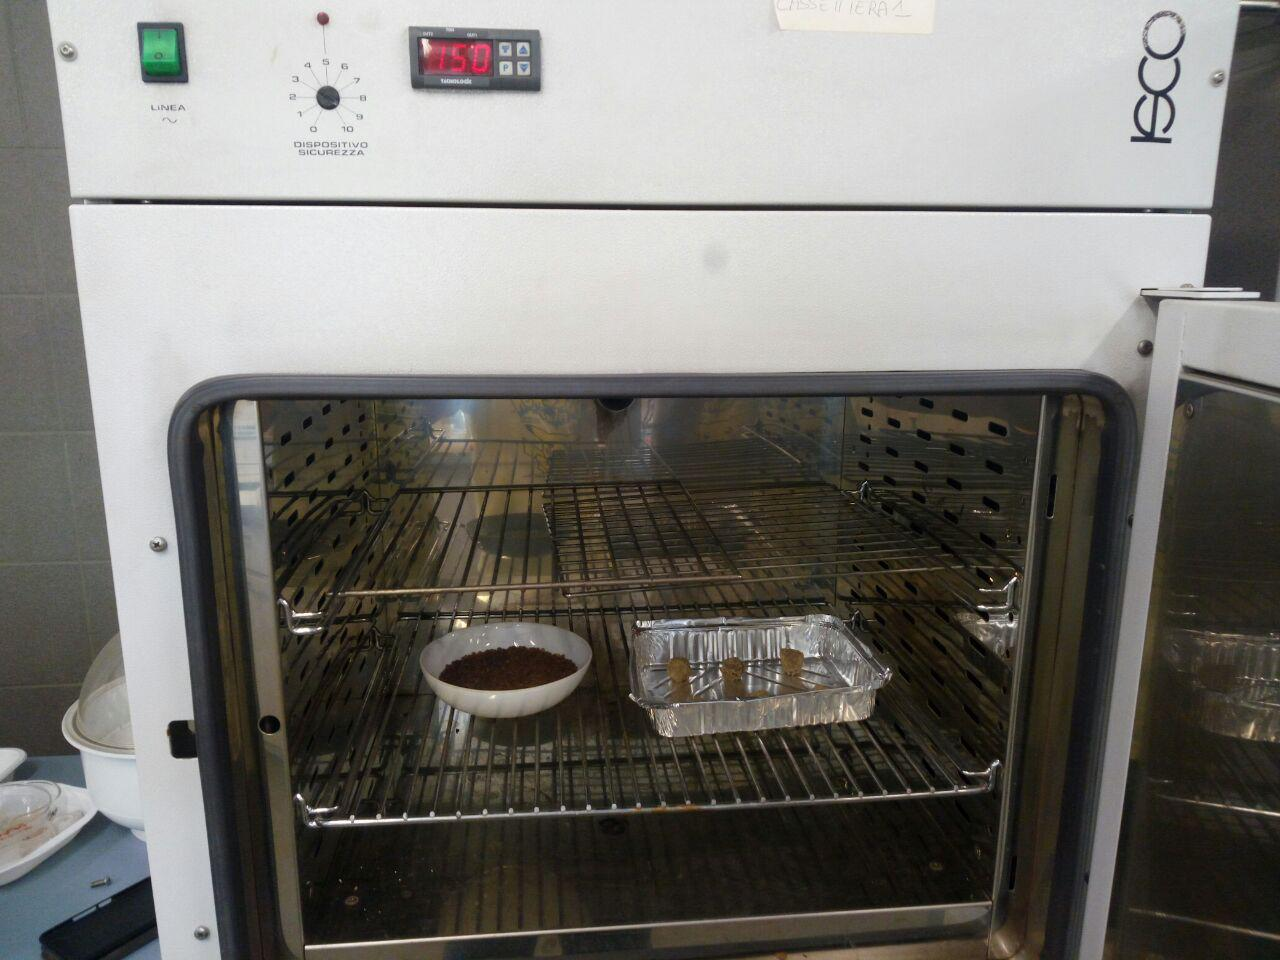
\includegraphics[width=0.8\textwidth]{../foto/fornospinta.jpeg}
      \end{figure}
    }
    \only<7>{
      \begin{center}
        \[
        D_{app} = \frac{P_{150}}{V_{aggregato}}
        \]
      \end{center}
    }
  \end{columns}
\end{frame}



\begin{frame}
  % latex table generated in R 3.4.0 by xtable 1.8-2 package
  % Thu Jun 22 16:26:59 2017
  \footnotesize
  \begin{table}[ht]
    \centering
    \begin{tabular}{rrccc}
      \hline
      Conduzione & Lavorazione & densit\`a apparente $g/cm^3$& Dev. std & n \\ 
      \hline
      CO & Ara & 1.93 & 0.11 &  18 \\ 
                 & Fzo & 1.87 & 0.06 &  18 \\ 
                 & Rip & 1.88 & 0.09 &  18 \\ \\
      OO & Ara & 1.91 & 0.13 &  18 \\ 
                 & Fzo & 1.82 & 0.07 &  18 \\ 
                 & Rip & 1.85 & 0.14 &  18 \\ 
      \hline
    \end{tabular}
    \label{tab:RiassuntoDensitaSpinta}
  \end{table}
\end{frame}

\begin{frame}
  \transdissolve<2>
  \begin{figure}
    \only<1>{
      \includegraphics[width=0.8\textwidth]{../grafici/density/boxplot_campo2016.pdf}
    }
    \only<2>{
      \includegraphics[width=0.8\textwidth]{../grafici/density/boxplot_petrolio.pdf}
    }
  \end{figure}
\end{frame}

\begin{frame}{Tabella Anova  densit\`a piccoli aggregati}
  % latex table generated in R 3.4.0 by xtable 1.8-2 package
  % Thu Jun 22 16:32:35 2017
  \begin{table}
    \centering
    \begin{tabular}{lrrrrr}
      \hline
      & Df & Sum Sq & Mean Sq & F value & Pr($>$F) \\ 
      \hline
      Conduzione & 1 & 0.03 & 0.03 & 6.31 & 0.012 \\ 
      Lavorazione & 2 & 0.05 & 0.02 & 5.83 & 0.004 \\ 
      Residui & 104 & 0.42 & 0.00 &  &  \\ 
      \hline
    \end{tabular}
    \label{tab:Anova densita per spinta}
  \end{table}
\end{frame}

% \begin{frame}
%   \begin{figure}[ht]
%     \includegraphics[width=0.8\textwidth]{../grafici/density/plot_petrolio.pdf}
%   \end{figure}
% \end{frame}

\begin{frame}{t-table  densit\`a piccoli aggregati}
  % latex table generated in R 3.4.0 by xtable 1.8-2 package
  % Thu Jun 22 10:44:00 2017
  \footnotesize
  % latex table generated in R 3.4.0 by xtable 1.8-2 package
  % Thu Jun 22 16:31:31 2017
  \begin{table}[ht]
    \centering
    \begin{tabular}{rrrrr}
      \hline
      & Estimate & Std. Error & t value & Pr($>$$|$t$|$) \\ 
      \hline
      % Convenzionale arato & 1.9470 & 0.0295 & 65.98 & 0.0000 \\ 
      % Scostamento biologico & -0.0534 & 0.0295 & -1.81 & 0.0731 \\ 
      % Scostamento frangizollato & -0.0780 & 0.0361 & -2.16 & 0.0331 \\ 
      % Scostamento rippato & -0.0881 & 0.0361 & -2.44 & 0.0164 \\ 
      Convenzionale arato & 1.93 & 0.01 & 157.38 & 0.000 \\ 
      Scostamento biologico & -0.03 & 0.01 & -2.51 & 0.014 \\ 
      Scostamento frangizollato & -0.05 & 0.02 & -3.39 & 0.001 \\ 
      Scostamento rippato & -0.03 & 0.02 & -2.04 & 0.043 \\ 
      \hline
    \end{tabular}
    \label{tab:Riassunto densita spinta}
  \end{table}
\end{frame}



\part{Stabilit\`a degli aggregati}
% \section{Strumentazione e metodo}
\begin{frame}
  \frametitle{Misura stabilit\`a degli aggregati}
  % \citep{ugolini2010basi} 
  \begin{columns}
    \column{.50\textwidth}
    % \begin{block}{}
    \pause
    \begin{enumerate}[<+->] 
    \item separazione della frazione compresa tra 1 e 2 mm  
    \item 300 mg di campione (secco a \SI{40}{\celsius}) vengono immessi
      nel vasca di misura piena d'acqua dello strumento Hydro 2000g
    \item acquisizione temporale della distribuzione granulometrica:
      una al minuto per 12 minuti durante i quali \ldots
    \item lo strumento provvede al ricircolo dell'acqua che disgrega
      le particelle di suolo
    \item attivazione della sonicazione dal \SI{13}{\degree} al
      \SI{24}{\degree} minuto per completare la rottura degli
      aggregati
      
    \end{enumerate}
    % \end{block}
    \column{.48\textwidth}
    \only<3>{
      \begin{figure}[ht]
        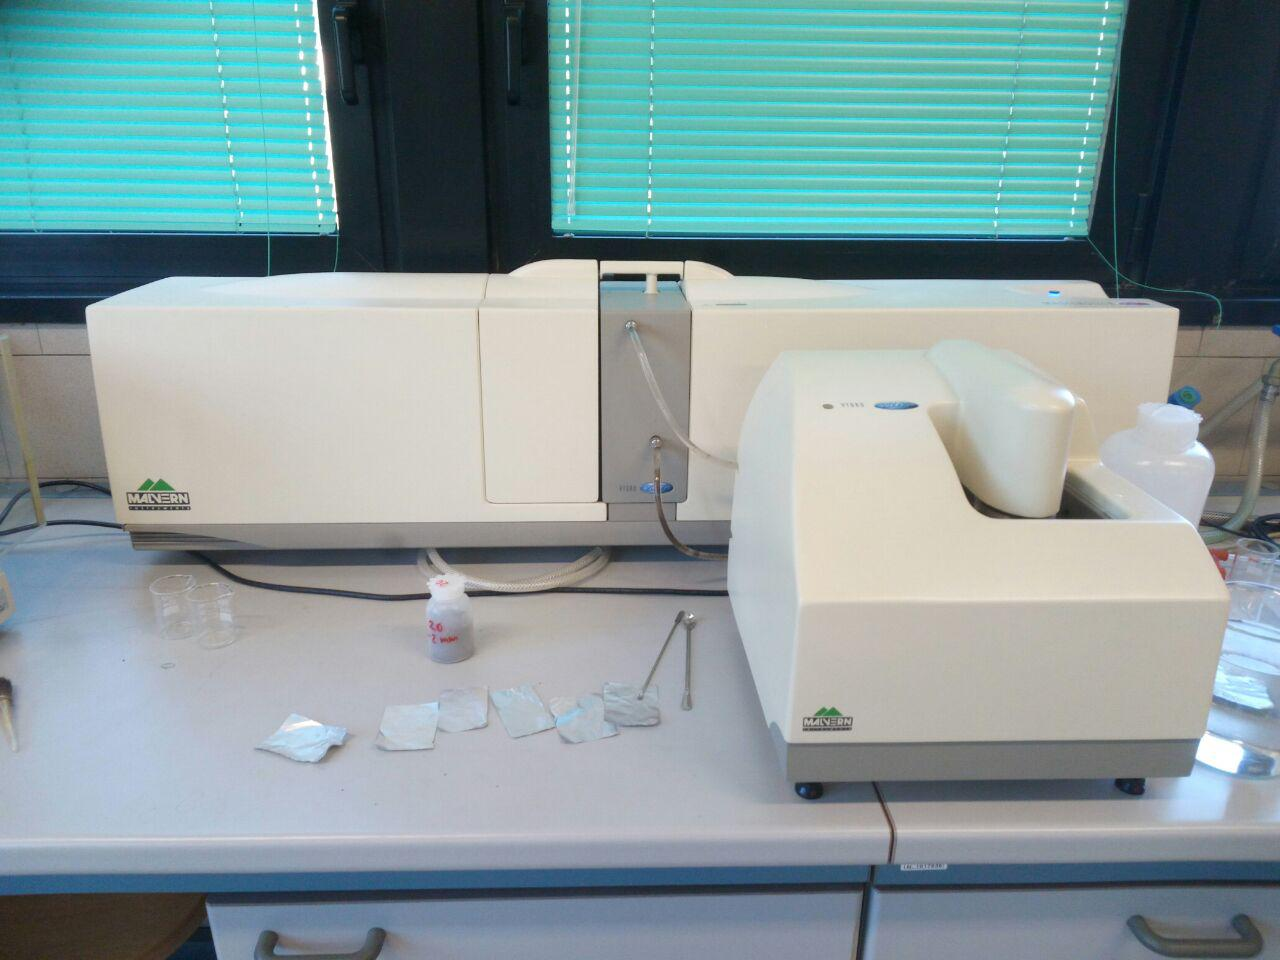
\includegraphics[width=\textwidth]{../foto/Hydro.jpeg}
      \end{figure}
    }
    \only<4->{
      \begin{figure}[ht]
        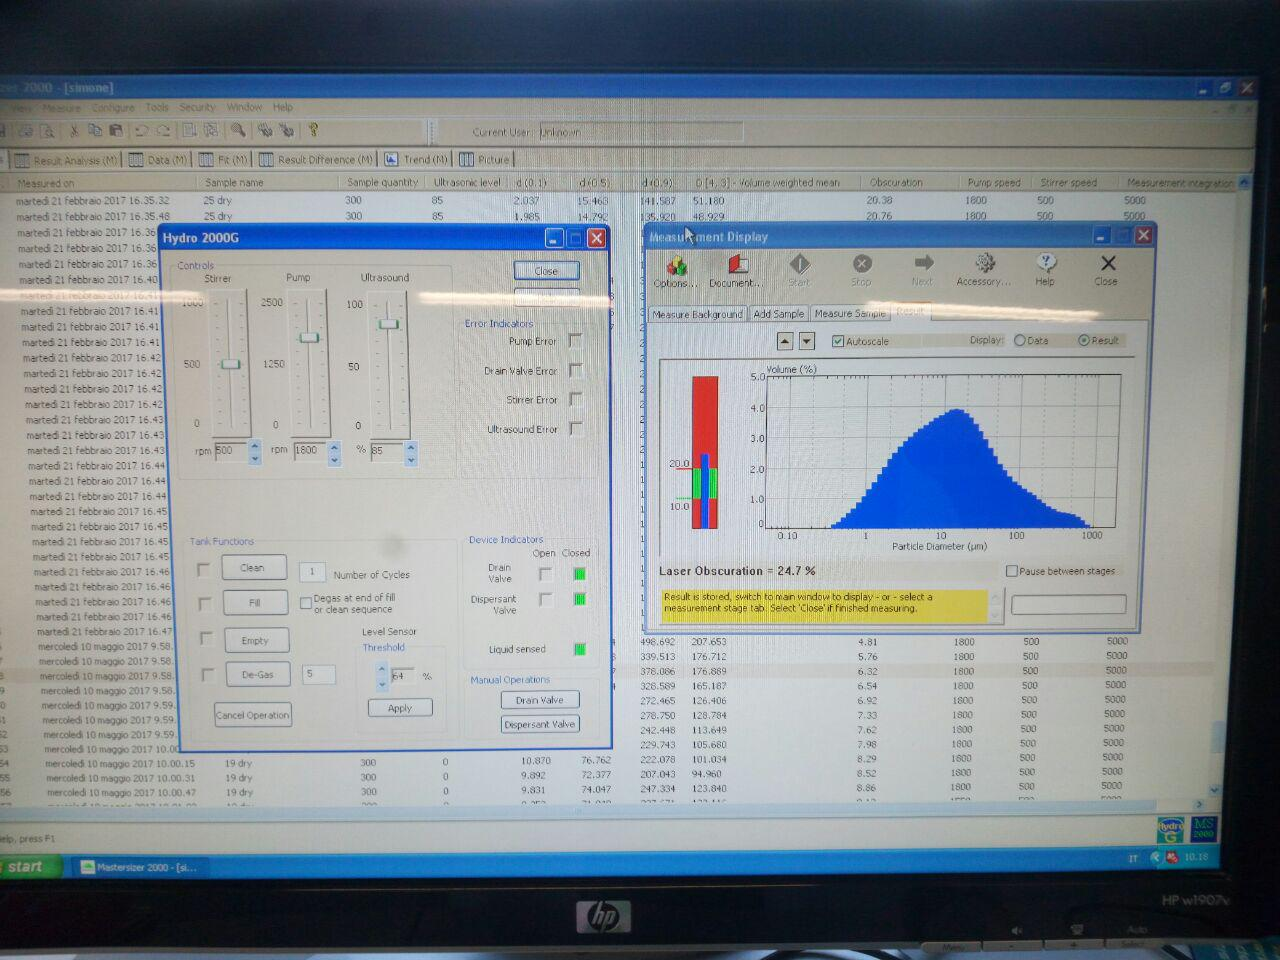
\includegraphics[width=\textwidth]{../foto/Acquisiz.jpeg}
      \end{figure}
    }
  \end{columns}  

\end{frame}

\begin{frame}
  \footnotesize
  \begin{itemize}
  \item La variazione della distribuzione nel tempo ci fornisce
    informazioni sulla resistenza degli aggregati alle sollecitazioni
    meccaniche.
  \item Oltre che sui campioni \textcolor{blue}{secchi}, la misura
    \`e stata ripetuta su aggregati 
    \textcolor{magenta}{previamente inumiditi} per evitare lo \textit{slacking}
  \end{itemize}

  \begin{figure}
    \includegraphics[width=0.6\textwidth, page=6]{../grafici/PISA2.pdf}
  \end{figure}
\end{frame}

\begin{frame}
  \begin{figure}
    \includegraphics[width=0.9\textwidth, page=1]{../grafici/UltrasuoniSI_NO_UMIDITA_WET_DRY.pdf}
  \end{figure}
\end{frame}

\begin{frame}{Tabella Anova dati composizionali}
\footnotesize
  % latex table generated in R 3.4.0 by xtable 1.8-2 package
  % Tue Jun 27 21:29:19 2017
  \begin{table}
    \centering
    \begin{tabular}{lrrrrrr}
      \hline
      & Df & Pillai & approx F & num Df & den Df & Pr($>$F) \\ 
      \hline
      COnvenzionale & 1 & 0.92 & 4955.26 & 2 & 835 & $<10^{-3}$ \\ 
      Organico  & 1 & 0.09 & 41.72 & 2 & 835 &  $<10^{-3}$ \\ 
      Tempo & 1 & 0.92 & 4504.77 & 2 & 835 &  $<10^{-3}$  \\ 
      Tempo$^2$& 1 & 0.35 & 227.06 & 2 & 835 &  $<10^{-3}$ \\ 
      Residui & 836 &  &  &  &  &  \\ 
      \hline
    \end{tabular}
  \end{table}
\end{frame}




\part{Penetrometria}

\begin{frame}
  \begin{figure}[ht]
    \includegraphics[width=0.8\textwidth, page=1]{../grafici/penetrometria/Penetrometria2015-2016.pdf}
  \end{figure}
\end{frame}

\begin{frame}{Attenzione alla scala dell'asse y !!}
  \transdissolve<2->
  \begin{columns}
    \column{.65\textwidth}
    \begin{figure}
      \only<1-2>{
        $\sum\limits_{cm=0}^{cm=80}q_c$ %http://www.nrcresearchpress.com/doi/pdf/10.1139/cgj-2016-0156
        \includegraphics[width=0.9\textwidth,
        page=4]{../grafici/penetrometria/Penetrometria2015-2016.pdf}
      }
      \only<3>{
        $\sum\limits_{cm=0}^{cm=20}q_c$
        \includegraphics[width=0.9\textwidth,
        page=5]{../grafici/penetrometria/Penetrometria2015-2016.pdf}
      }
      \only<4>{
        $\sum\limits_{cm=20}^{cm=40}q_c$
        \includegraphics[width=0.9\textwidth, page=6]{../grafici/penetrometria/Penetrometria2015-2016.pdf}
      }
      \only<5>{
        $\sum\limits_{cm=40}^{cm=80}q_c$
        \includegraphics[width=0.9\textwidth, page=7]{../grafici/penetrometria/Penetrometria2015-2016.pdf}
      }
    \end{figure}
    \column{.33\textwidth}
    
    \begin{itemize}[<+->]
      \small    
    \item differenza, sia per valori assoluti che per varianza, tra le
      due sessioni dovute a diverse condizioni di misura (operatori,
      condizioni di campo)
    \item suddivisione in tre diversi range di profondit\`a:
      \begin{itemize}
      \item effetto anno attenuato (CO.Fzo pi\`u duro) %0-20cm
      \item anche qui come sopra       %\item 20-40 cm
      \item in profondit\`a la varianza si
        attenua %40-80 cm
      \end{itemize}
    \end{itemize}
  \end{columns}
\end{frame}

\begin{frame}
  \begin{figure}[ht]
    \includegraphics[width=0.8\textwidth, page=8]{../grafici/penetrometria/Penetrometria2015-2016.pdf}
  \end{figure}
\end{frame}


\begin{frame}
  \begin{figure}[ht]
    \includegraphics[width=0.8\textwidth, page=9]{../grafici/penetrometria/Penetrometria2015-2016.pdf}
  \end{figure}
\end{frame}

\begin{frame}
  \begin{figure}[ht]
    \includegraphics[width=0.8\textwidth, page=10]{../grafici/penetrometria/Penetrometria2015-2016.pdf}
  \end{figure}
\end{frame}

\begin{frame}{Sintesi finale}
  \begin{itemize}[<+->]
  \item La densit\`a per grandi volumi mostra una maggior compattezza
    negli appezzamenti OO. Differenza significativa, ma solo sulla
    seconda cifra decimale. Nessun effetto delle lavorazioni
  \item La densit\`a misurata sugli aggregati mostra l'inverso (OO
    meno compatto). Anche qui differenze sulla seconda decimale. Le
    lavorazioni mostrano un effetto (aratura la pi\`u compatta)
  \item Le misure di stabilit\`a indicano un suolo generalmente poco
    stabile (aggregati inferiori a 1 mm) e che il CO produce aggregati
    di maggiori dimensioni (sia secchi che umidi).
  \item La penetrometria indica un marcato effetto dell'anno (=
    sessione di misura) attribuibile alle condizioni meteo e agli
    operatori. L'appezzamento CO.F.zo risulta sempre pi\'u duro
    rispetto agli altri. Analisi composizionale dubbia.
    \item Porosimetria da analizzare
  \end{itemize}
  
\end{frame}



% \part{Porosimetria a mercurio}
\end{document}



%%% Local Variables:
%%% mode: latex
%%% TeX-master: t
%%% End:
